\documentclass{report}

\input{~/dev/latex/template/preamble.tex}
\input{~/dev/latex/template/macros.tex}

\title{\Huge{}}
\author{\huge{Nathan Warner}}
\date{\huge{}}
\pagestyle{fancy}
\fancyhf{}
\lhead{Warner \thepage}
\rhead{}
% \lhead{\leftmark}
\cfoot{\thepage}
\setborder
% \usepackage[default]{sourcecodepro}
% \usepackage[T1]{fontenc}

\begin{document}
    % \maketitle
        \begin{titlepage}
       \begin{center}
           \vspace*{1cm}
    
           \textbf{Chapters 1-4}
    
           \vspace{0.5cm}
           Stat 128: Elementary Statistics
            
                
           \vspace{1.5cm}
   
           A Document By: \\
           \textbf{Nathan Warner}
    
           \vfill
                
                
           \vspace{0.8cm}
         
           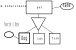
\includegraphics[width=0.4\textwidth]{./figures/2.png}
           \bigbreak \noindent 
            July 03, 2023  \\
           Computer Science \\
           Joliet Junior College \\
           United States\\
           
                
       \end{center}
    \end{titlepage}
    \tableofcontents
    \pagebreak \bigbreak \noindent
    \section{Learning Outcomes}
    \bigbreak \noindent 
    \textbf{Chapter 1:}
    \begin{enumerate}
        \item Define data collection techniques including observational studies and design of experiments.
        \item Identify appropriate sampling methods.
    \end{enumerate}
    \bigbreak \noindent 
    \textbf{Chapter 2:}
    \begin{enumerate}
        \item Differentiate qualitative and quantitative data graphically.  This includes graphs such as bar plots, histograms, and dot plots.
    \end{enumerate}
    \bigbreak \noindent 
    \textbf{Chapter 3:}
    \begin{enumerate}
        \item Calculate measures of central tendency for data.
        \item Explain the concept of resistance.
        \item Decide which measure of central tendency to report for various data sets.
        \item Determine measures of dispersion for data.
        \item Determine standard scores, percentiles, and quartiles.
        \item Identify outliers using quartiles.
        \item Interpret boxplots.
    \end{enumerate}
    \bigbreak \noindent 
    \textbf{Chapter 4:}
    \begin{enumerate}
        \item Evaluate the linear correlation coefficient for bivariate quantitative data.
        \item Evaluate whether the coefficient is significant at a given level.
        \item Explain the difference between correlation and causation.
        \item Determine the least-squares regression equation for a given set of bivariate data.
        \item Predict values of the dependent variable using the least-squares regression equation.
        \item Interpret the slope and intercept of the least-squares regression equation.
        \item Test the requirements of the least-squares regression model using residual analysis.
        \item Determine and interpret the coefficient of determination.
        \item Graphically analyze bivariate quantitative data for outliers and influential observations.
        \item Describe the association between two qualitative variables using conditional distributions.
        \item Explain Simpson’s Paradox.
    \end{enumerate}

    \pagebreak \bigbreak \noindent
    \section{Chapter 1:}

    \bigbreak \noindent 
    \subsection{1.1: Introduction to the Practice of Statistics}

    \bigbreak \noindent 
    \textbf{\textit{\underline{Objectives for this section.}}}
    \begin{enumerate}
        \item Define Statistics and Statistical Thinking
        \item Explain the Process of Statistics
        \item Distinguish between Qualitative and Quantitative Variables
        \item Distinguish Between Discrete and Continuous Variables.
    \end{enumerate}
    
    \bigbreak \noindent \bigbreak \noindent 
    \textbf{\textit{\underline{Define Statistics and Statistical Thinking:}}}
    \bigbreak \noindent
        Statistics is the science of collecting, organizing, summarizing, and analyzing information to draw conclusions or answer questions. In addition, statistics is about providing a measure of confidence in any conclusions.
        \bigbreak \noindent 
        \textbf{Note:} We must report a measure of our confidence in our results because we do not have 100\% certainty our answers are correct.
        \bigbreak \noindent 
        The information referred to in the definition above is \textit{data}. \textbf{Data} are a "fact or proposition used to draw a conclusion or make a decision." Data describes characteristics of an individual.
        \bigbreak \noindent 
        One crucial thing to understand about \textbf{data}, is that is \textbf{varies}. One thing that makes an interesting study is the fact that the data within the study varies. A study about number of hearts a human has is not only uninteresting but not worth doing. This is because the data does not vary.
        \bigbreak \noindent 
        \textbf{Two Major Goals:}
        \begin{enumerate}
            \item Describe Variability.
            \item Understand sources of Variability.
        \end{enumerate}
        \bigbreak \noindent 
        In Statistics, the same approach to solving a problem can still lead to different results. This does not happen in a math class.
        \vspace{1em}

        \bigbreak \noindent \bigbreak \noindent 
        \textbf{\textit{\underline{Explain the Process of Statistics.}}}
        \bigbreak \noindent 
        First lets define some vocabulary:
        \begin{itemize}
            \item \textbf{Population:} The entire group to be studied is called the population.
            \item \textbf{Sample:} In statistics, it is often impractical or impossible to get access to the entire \textbf{population}, which is why we only look at a \textbf{sample.} A sample is a \textbf{subset} of the population being studied.
            \item \textbf{Individual:} An individual is a person or object that is a member of the population being studied.
            \item \textbf{Statistic:} A statistic is a numerical summary of a sample.
            \item \textbf{Descriptive Statistics:} Descriptive statistics consist of organizing and summarizing data. Descriptive statistics describe data through numerical summaries, tables, and graphs.
            \item \textbf{Inferential Statistics:} inferential Statistics uses methods that take a result from a sample, extend it to the population, and measure the reliability of the result.
            \item \textbf{Parameter:} A parameter is a numerical summary of a population.
        \end{itemize}

        \bigbreak \noindent 
        \textbf{The process of statistics:}
        \begin{enumerate}
            \item Identify the problem to be solved. It is important to clearly lay out the questions that the researcher wants answered, along with clearly specifying which population the study applies.
            \item Collect the data.
            \item Describe the data.
            \item Preform inference.
        \end{enumerate}

        \bigbreak \noindent 
        \begin{mdframed}
          \textbf{Example: The AP - National Constitution Center conducted a national poll to learn how adult Americans feel existing gun-control laws infringe on the second amendment to the U.S Constitution}
          \bigbreak \noindent 
          \textbf{The Following statistical process allowed the researchers to conduct their study.}
          \begin{enumerate}
              \item \textbf{Identify the research objective.}: The researchers wished to determine the percentage of adult Americans who believe gun-control laws infringe on the public's right to bear arms.
            \item \textbf{Collect the information needed to answer the question posed in (1).}: It is unreasonable to expect to survey the more than 200 million adult Americans to determine how they feel about gun-control laws. So the researchers surveyed a sample of 1007 adult Americans. Of those surveyed, 514 stated they believe existing gun-control laws infringe on the public's right to bear arms.
            \item \textbf{Describe the data.}: Of the 1007 individuals in the survey, 51\% believe existing gun-control laws inferring on the public's right to bear arms. This is a descriptive statistic, because its value is determined from a sample.
            \item \textbf{Preform inference.}: The researchers at the AP - National Constitution Center wanted to extend the results of the survey to \textbf{all} adult Americans. When generalizing results from a sample to a population, the results are \textbf{uncertain}. To account for this uncertainty, researchers reported a 3\% \textit{margin of error.} This means that the researchers feel fairly certain (in fact, 95\% certain) that the percentage of \textit{all} adult Americans who believe existing gun-control laws infringe on the public's right to bear arms is somewhere between 48\% and 54\%

          \end{enumerate}
          
        \end{mdframed}

        \bigbreak \noindent \bigbreak \noindent 
        \textbf{\textit{\underline{Distinguish between Qualitative and Quantitative Variables}}}
        \bigbreak \noindent 
        First let's define some vocab:
        \begin{itemize}
            \item \textbf{Variables:} The characteristics of the individuals in a study. Variables vary, which means they can take on different values.
            \item \textbf{Constants:} Variables that do not vary. Inferential statistics is not necessary with constants.
        \end{itemize}
        \bigbreak \noindent 
        One goal of research is to learn the causes of variability.
        \bigbreak \noindent 
        Variables can be classified into two groups: qualitative and quantitative.
        \begin{itemize}
            \item \textbf{Qualitative, or categorical variables} allow for the classification of individuals base on some attribute or characteristic.
            \item \textbf{Quantitative variables} provide numerical measures of individuals. The values of a quantitative variable can be added or subtracted and provide meaningful results.
        \end{itemize}
        \bigbreak \noindent 
        \begin{mdframed}
          \textbf{Example: Determine whether the following variables are qualitative or quantitative.}
          \begin{enumerate}[label=\alph*.)]
              \item \textbf{Gender.}: Qualitative
              \item \textbf{Temperature.}: Quantitative
              \item \textbf{Number of days during the past week that a college student studied.}: Quantitative
              \item \textbf{Zip Code.} Qualitative
          \end{enumerate}
          \textbf{Caution:} A numeric value does not automatically suggest a variable is quantitative.
        \end{mdframed}

        \bigbreak \noindent 
        \textbf{\textit{\underline{Distinguish between Discrete and Continuous Variables.}}}
        \begin{itemize}
            \item A \textbf{discrete variable} is a quantitative variable that has either a finite number of possible values or a countable number of possible values. A discrete variable cannot take on every possible value between any two possible values.
            \item A \textbf{continuous variable} is a quantitative variable that has an infinite number of possible values that are not countable. A continuous variable may take on every possible value between any two values. Continuous variables typically result from measurement. Continuous variables are often rounded. If a certain make of car gets 24 miles per gallon (mpg) of gasoline, its miles per gallon must be greater than or equal to 23.5 and less than 24.5, or $23.5 \leq mpg \leq 24.5$
        \end{itemize}

        \bigbreak \noindent 
        This Figure illustrates the relationship among qualitative, quantitative, discrete, and continuous variables.

        \begin{figure}[ht]
            \centering
            \incfig{graph1}
            \label{fig:graph1}
        \end{figure}

        \bigbreak \noindent 
        \begin{mdframed}
          \textbf{Example: Distinguish whether the quantitative variables are discrete or continuous.}
          \begin{enumerate}[label=\alph*.)]
            \item \textbf{The number of heads obtained after flipping a coin five times.}: Discrete
            \item \textbf{The number of cars that arrive at a McDonald's drive through between 12:00 PM and 1:00 PM}: Discrete
            \item \textbf{The Distance a 2011 Toyota Prius can travel in city driving conditions with a full tank of gas.}: Continuous
          \end{enumerate}
        \end{mdframed}

        \bigbreak \noindent 
        \textbf{Vocab:}
        \begin{itemize}
            \item The list of observed values for a variable is \textbf{data.}
            \item \textbf{Qualitative data} are observations corresponding to a \textbf{qualitative variable.}
            \item \textbf{Quantitative data} are observations corresponding to a quantitative variable.
            \item \textbf{Discrete data} are observations corresponding to a discrete variable.
            \item \textbf{Continuous data} are observations corresponding to a continuous variable.
        \end{itemize}

        \bigbreak \noindent 
        \begin{mdframed}
          \textbf{Example: Distinguish between Variables and Data}
          \bigbreak \noindent 
          The following table presents a group of selected countries and information regarding these countries.
          \bigbreak \noindent 
          Identify the individuals, variables, and data.
          \begin{center}
              \begin{tabular}{|l|c|c|c|}
              \hline
              Country & Government Type & Life Expectancy (Years) & Population (in millions) \\
              	\hline
              Australia & Federal parliamentary democracy & 81.63 & 21.3   \\
              	\hline
            Canada & Constitutional monarchy & 81.23 & 33.5 \\
            \hline
            France & Republic & 80.98 & 64.4 \\
            \hline
            Morocco & Constitutional monarchy & 75.47 & 31.3 \\
            \hline
            Poland & Republic & 75.63 & 38.5 \\
            \hline
            Sri Lanka & Republic & 75.14 & 21.3\\
            \hline
            United States & Federal Republic & 78.11 & 307.2 \\
            \hline
              \end{tabular}
          \end{center}
          \bigbreak \noindent 
          \textbf{Qualitative}: Government Type \\
          \textbf{Quantitative}: Life Expectancy and Population \\
          \textbf{Continuous}: Life Expectancy \\
          \textbf{Discrete}: Population \\
          \textbf{Data}: Everything under Government Type, Life Expectancy, and Population.
      \item 
        \end{mdframed}

        \pagebreak \bigbreak \noindent
        \begin{center}
            \begin{large}
                \textbf{All Vocab / Concepts From Section 1.1}
            \end{large}
        \end{center}
        \line(1,0){490}
        \begin{itemize}
            \item \textbf{Population:} The entire group to be studied is called the population.
            \item \textbf{Sample:} In statistics, it is often impractical or impossible to get access to the entire \textbf{population}, which is why we only look at a \textbf{sample.} A sample is a \textbf{subset} of the population being studied.
            \item \textbf{Individual:} An individual is a person or object that is a member of the population being studied.
            \item \textbf{Statistic:} A statistic is a numerical summary of a sample.
            \item \textbf{Descriptive Statistics:} Descriptive statistics consist of organizing and summarizing data. Descriptive statistics describe data through numerical summaries, tables, and graphs.
            \item \textbf{Inferential Statistics:} inferential Statistics uses methods that take a result from a sample, extend it to the population, and measure the reliability of the result.
            \item \textbf{Parameter:} A parameter is a numerical summary of a population.
            \item \textbf{Variables:} The characteristics of the individuals in a study. Variables vary, which means they can take on different values.
            \item \textbf{Constants:} Variables that do not vary. Inferential statistics is not necessary with constants.
            \item \textbf{Data:} The list of observed values for a variable.
            \item \textbf{Qualitative data} are observations corresponding to a \textbf{qualitative variable.}
            \item \textbf{Quantitative data} are observations corresponding to a quantitative variable.
            \item \textbf{Discrete data} are observations corresponding to a discrete variable.
            \item \textbf{Continuous data} are observations corresponding to a continuous variable.
        \end{itemize}

        \bigbreak \noindent 
        \textbf{Concepts:}
        \begin{itemize}
            \item Statistics and Statistical Thinking.
            \item Describe Variability
            \item Understand Sources of variability
            \item Statistical studies are concerned with both describing the variability in the data and understanding the sources of variability in data. Understanding the sources allows researchers to control it and reach better conclusions.
            \item The process of statistics
            \item Inferential/Descriptive Statistics
            \item Variables
                \begin{itemize}
                    \item Qualitative (Categorical) / Quantitative
                    \item Discrete / Continuous
                \end{itemize}
            \item Data
                \begin{itemize}
                    \item Qualitative (Categorical) / Quantitative
                    \item Discrete / Continuous
                \end{itemize}
        \end{itemize}

        \pagebreak \bigbreak \noindent
        \subsection{1.2: Observational Studies versus Designed Experiments}
        \bigbreak \noindent 
        \textbf{\textit{\underline{Objectives for this section.}}}
        \begin{enumerate}
            \item Distinguish between an Observational Study and a Designed Experiment
            \item Explain the Various Types of Observational Studies
        \end{enumerate}

        \bigbreak \noindent 
        \textbf{\textit{\underline{Distinguish between an Observational Study and a Designed Experiment}}}
        \begin{itemize}
            \item \textbf{Observational studies:} Observational studies involve observing and analyzing data collected from real-world settings without any intervention or manipulation by the researcher. Researchers passively observe and record information to identify correlations or associations between variables.
            \item \textbf{Designed experiments:} Designed experiments, also known as randomized controlled trials (RCTs), involve researchers actively manipulating variables and randomly assigning participants to different groups. This allows researchers to establish cause-and-effect relationships by comparing the effects of different interventions or treatments on the outcome of interest.
        \end{itemize}
        \bigbreak \noindent 
        \textbf{Vocab:}
        \begin{itemize}
            \item \textbf{Explanatory Variable:} An explanatory variable, also known as an independent variable or predictor variable, is a variable that is manipulated or controlled by researchers in an experiment or study. It is the variable that is hypothesized to have an impact on the outcome or dependent variable. 
            \item \textbf{Lurking variable}: An explanatory variable that was not considered in a study, but that affects the value of the response variable.
            \item \textbf{Response Variable}: The response variable, also known as the dependent variable or outcome variable, is the variable that is measured or observed to determine the effect or response of the explanatory variable(s). It is the variable that researchers are interested in studying or predicting. 
            \item \textbf{Confounding:} Occurs when the effects of two or more explanatory variables are not separated. Therefore, any relation that may exist between an explanatory variable and the response variable may be due to some other variable or variables not accounted for in the study.
            \item \textbf{Census:} List of individuals in a population along with certain characteristics of each individual.
        \end{itemize}

        \bigbreak \noindent 
        \nt{Is observational studies, we \textbf{are not} allowed to make statements of \textit{causality}, meaning we cannot say that changes in the explanatory variable \textit{cause} changes in the response variable. We can only say changes in the explanatory variable are associated with changes in the response variable.}

        \bigbreak \noindent 
        Why would we ever conduct an observational study if we cannot claim causation? Because it is often unethical to conduct a designed experiment.
        \bigbreak \noindent 
        Consider the link between smoking and lung cancer. In a designed experiment (on humans) to determine if smoking causes lung cancer, a researcher would divide a group of volunteers into two groups—Group 1 would smoke a pack of cigarettes every day for the next 10 years, and Group 2 would not smoke. Eating habits, sleeping habits, and exercise would be controlled so that the only difference between the two groups would be smoking. After 10 years, the experiment's researcher would compare the proportion of participants in the study who contract lung cancer in the smoking group with the nonsmoking group. If the two proportions differ significantly, it could be said that smoking causes lung cancer. This designed experiment controls many potential cancer-causing factors that would not be controlled in an observational study. However, it is an unethical experiment. Do you see why?
        \bigbreak \noindent Other reasons exist for conducting observational studies over designed experiments. An article in support of observational studies states, "Observational studies have several advantages over designed experiments, including lower cost, greater timeliness, and a broader range of patients." From Kjell Benson, BA, and Arthur J. Hartz, MD, PhD. "A Comparison of Observational Studies and Randomized Controlled Trials." 

        \bigbreak \noindent 
        In designed experiments, it is possible to have two explanatory variables in a study that are related to each other and related to the response variable. For example, suppose Professor Egner wanted to conduct an experiment in which she compared student success using online homework versus traditional textbook homework. To do the study, she taught her morning statistics class using the online homework and her afternoon class using traditional textbook homework. At the end of the semester, she compared the final exam scores for the online section to the textbook section. If the morning section had higher scores, could Professor Egner conclude that online homework is the cause of higher exam scores? Not necessarily. It is possible that the morning class had students who were more motivated. It is impossible to know whether the outcome was due to the online homework or to the time at which the class was taught. In this sense, we say that the time of day the class is taught is a confounding variable.

        \bigbreak \noindent 
        \textbf{Lurking Vs Confounding Variables:}
        \bigbreak \noindent 
        The big difference between lurking variables and confounding variables is that lurking variables are not considered in the study (for example, we did not consider lifestyle in the pneumonia study) whereas confounding variables are measured in the study (for example, we measured morning versus afternoon classes).
        \bigbreak \noindent 
        So lurking variables are related to both the explanatory and response variables, and this relation is what creates the apparent association between the explanatory variable and response variable in the study. For example, lifestyle (healthy or not) is associated with the likelihood of getting an influenza shot as well as the likelihood of contracting pneumonia or influenza.
        \bigbreak \noindent 
        A confounding variable is a variable in a study that does not necessarily have any association with the other explanatory variable but does have an effect on the response variable. Perhaps morning students are more motivated, and this is what led to the higher final exam scores, not the homework delivery system.
        \bigbreak \noindent 
        The bottom line is that both lurking variables and confounding variables can confound the results of a study, so a researcher should be mindful of their potential existence.

        \bigbreak \noindent \bigbreak \noindent 
        \textbf{\textit{\underline{Explain the Various Types of Observational Studies}}}
        \bigbreak \noindent 
        \begin{itemize}
            \item \textbf{Cross-sectional Studies:} Observational studies that collect information about individuals at a specific point in time, or over a very short period of time.
            \item \textbf{case-control Studies:} These studies are \textbf{retrospective,} meaning that they require individuals to look back in time or require the researcher to look at existing records. In case-control studies, individuals that have certain characteristics are matched with those that do not.
                \begin{itemize}
                    \item \textbf{Positive:} Control group allows for a comparison
                    \item \textbf{Negative:} Individuals must remember details
                    \item \textbf{Negative:} Records might not exist
                \end{itemize}
            \item \textbf{Cohort Studies:} A cohort study first identifies a group of individuals to participate in the study (cohort). The cohort is then observed over a period of time. Over this time period, characteristics about the individuals are recorded. Because the data is collected over time, cohort studies are \textbf{prospective.}
                \begin{itemize}
                    \item \textbf{Advantage:} Researcher does not need to rely on memory of study participants or existing records.
                    \item \textbf{Disadvantage:} Requires a lot of time.
                    \item \textbf{Disadvantage:} Could be expensive.
                \end{itemize}
        \end{itemize}

        \pagebreak \bigbreak \noindent
        \textbf{Is a designed experiment superior to an observational study? Not necessarily.}
        \begin{itemize}
            \item Because cross-sectional and case-control observational studies are relatively inexpensive, they allow researchers to explore possible associations prior to undertaking large cohort studies or designed experiments.
            \item It is not always possible to conduct an experiment. For example, we could not conduct an experiment to investigate the perceived link between high-tension wires and leukemia (on humans). Do you see why?
        \end{itemize}

        \pagebreak \bigbreak \noindent
        \subsection{1.3: Simple Random Sampling}
        \bigbreak \noindent 
        \textbf{\textit{\underline{Learning Objectives for this section.}}}
        \begin{enumerate}
            \item Obtain a simple random sample
        \end{enumerate}
        \bigbreak \noindent 
        \textbf{Vocab:}
        \begin{itemize}
            \item \textbf{Random Sampling:} The process of using chance to select individuals from a population to be included in the sample.
            \item \textbf{Simple Random Sampling:} A sample of size $n$  from a population of size $N $  is obtained through simple random sampling if every possible sample of size $n$  has an equal chance of occurring. The sample is then called a simple random sample.
                \begin{itemize}
                    \item $n < N $
                \end{itemize}
            \item \textbf{frame:} a list of all the individuals within the population.
        \end{itemize}

        \bigbreak \noindent 
        \nt{For the results of a survey to be reliable, the characteristics of the individuals in the sample must be representative of the characteristics of the individuals in the population. The key to obtaining a sample representative of a population is to let chance or randomness, rather than convenience, play a role in dictating which individuals are in the sample. If convenience is used to obtain a sample, the results of the survey are meaningless.}

        \bigbreak \noindent 
        \textbf{Recognizing a Convenience Sample and Its Limitations:}
        \bigbreak \noindent 
        Suppose that Gallup wants to know the proportion of adult Americans who consider themselves to be baseball fans. If Gallup obtained a sample by standing outside Fenway Park (home of the Boston Red Sox professional baseball team), the survey results are not likely to be reliable. Why? Clearly, the individuals in the sample do not accurately reflect the makeup of the entire population.
        \bigbreak \noindent 
        Suppose you wanted to learn the proportion of students on your campus who work. It might be convenient to survey the students in your statistics class, but do these students represent the overall student body? Does the proportion of freshmen, sophomores, juniors, and seniors in your class mirror the proportion of freshmen, sophomores, juniors, and seniors on campus? Does the proportion of males and females in your class resemble the proportion of males and females across campus? Probably not. What about evening (or day) students? For these (and many other) reasons, the convenient sample is not representative of the population, which means that any results reported from your survey are misleading.

        \bigbreak \noindent 
        \textbf{Effective Sampling Techniques:}
        \begin{enumerate}
            \item \tetxbf{Simple random sampling}
            \item \tetxbf{Stratified sampling}
            \item \tetxbf{Systematic sampling}
            \item \tetxbf{Cluster sampling}
        \end{enumerate}
        \bigbreak \noindent 
        These sampling methods are designed so that any selection biases the surveyor introduced (knowingly or unknowingly) during the selection process are eliminated. In other words, the surveyor does not have a choice as to which individuals are in the study. We will discuss simple random sampling in this section and the remaining three types of sampling in the next section.

        \bigbreak \noindent 
        \begin{mdframed}
          \textbf{Bonus: Consider a set of 5 possibilities A-E, and we want to determine the total number of combinations of selecting 3 letters:}
          \bigbreak \noindent 
          We can use the formula:
          \begin{align*}
              nCk = \frac{n!}{(k!(n-k)!)}
          .\end{align*}
          \bigbreak \noindent 
          Where $n $ is the total number of classes in the course list and $k$ is the number of classes to be chosen.
          \bigbreak \noindent 
          So we have $n =5$ and $k = 3$:
          \begin{align*}
                \frac{5!}{(3!(5-3)!)} \\
                = \frac{5!}{3! \cdot 2!}\\
                 = \frac{5 \cdot 4 \cdot 3!}{3! \cdot 2\cdot 1} \\
                 = \frac{5 \cdot 4}{2\cdot 1} \\
                 = \frac{20}{2} \\
                 = 10
          .\end{align*}
          \bigbreak \noindent 
          And we can calculate the chance over a certain event happening with:
          \begin{align*}
              Probablility = \frac{Number of Occurences}{Total Number of Occurences}
          .\end{align*}
        \end{mdframed}

        \bigbreak \noindent 
        \textbf{How do we select the individuals in a simple random sample?}
        \bigbreak \noindent 
        We could write the names of the individuals in the population on different pieces of paper and then select names from a hat. Often, however, the size of the population is so large that performing simple random sampling in this fashion is not practical.
        \bigbreak \noindent 
        Typically, each individual in the population is assigned a unique number between 1 and $N$, Where $N$ is the size of the population. Then $n $ distinct random numbers are selected, where $n $ is the size of the population
        \bigbreak \noindent 
        To number the individuals in the population, we need a \textbf{frame:} a list of all the individuals within the population.

        \bigbreak \noindent 
        \textbf{Obtaining a simple random sample with calculator (ti-84)}
        \bigbreak \noindent 
        The accounting firm of Senese and Associates has grown. To make sure their clients are still satisfied with the services they are receiving, the company decides to send a survey out to a simple random sample of 5 of its 30 clients.
        \bigbreak \noindent 
        So we need 5 unique random numbers from a range of 1-30. To do this in our ti-84 calculator:
        \begin{enumerate}
            \item Math $\rightarrow$ Prod $\rightarrow$ randIntNorep
            \item Syntax: randIntNoRep(\textit{lowerbound}, \textit{upperbound}, \textit{$n$}), where $n$ is the number of unique random numbers we must generate.
            \item Lower: 1
            \item Upper: 30
            \item $n$: 5
            \item Select Paste.
        \end{enumerate}

        \pagebreak \bigbreak \noindent
        \subsection{1.4: Other Effective Sampling Methods}
        \bigbreak \noindent 
        \textbf{\textit{\underline{Learning Objectives}}}
        \begin{enumerate}
            \item \textbf{Obtain a Stratified Sample}
            \item \textbf{Obtain a Systematic Sample}
            \item \textbf{Obtain a Cluster Sample}
        \end{enumerate}
        \bigbreak \noindent 
        \textbf{Vocab:}










    
\end{document}
